\subsection{Larger candidate sets improve gradient approximation}
\label{sec:coverage_gradient}

Truncating vocabulary support omits probability mass and changes token weights \citep{anshumann2025sparse,huang2026tailaware}. We measure coverage as the student probability retained by the student--teacher candidate intersection, $c_k(h)=\sum_{v\in S\cap T}p_\theta(v\mid h)$, and compare gradients on identical inputs.

\paragraph{Top-64 closely matches the full-vocabulary direction in the Qwen measurements.}
The intersection retains over 99.9\% of student probability on average at the evaluated Qwen checkpoints. At these checkpoints, its gradient direction is close to that of full-vocabulary supervision (Figure~\ref{fig:supervision_overview}b). Sampled-token gradients become more aligned with the full-vocabulary direction as more token samples are averaged at each fixed prefix (Figure~\ref{fig:sampling_history_controls}a). This sampling control identifies finite-sample variation as one source of the directional difference.

\paragraph{Lower-coverage inputs retain appreciable gradient error in SmolLM.}
SmolLM3-3B measurements use a supervised initialization and a student trained with three domain teachers \citep{gao2026openmopddiagnosingfixingcapability}. Top-64 retains 97--99\% of student probability on average, with a subset of inputs retaining less than 90\% (Figure~\ref{fig:smollm_supervision}a,b). Larger candidate sets reduce the frequency of these low-coverage inputs.

On fixed inputs at the trained student, top-64 gradients have roughly 2--25\% relative error against full-vocabulary gradients. Top-4 and top-8 produce larger errors in the evaluated batches (Figure~\ref{fig:smollm_supervision}d). Here relative error is the norm of the gradient difference divided by the full-vocabulary gradient norm, capturing both direction and magnitude. Larger candidate sets improve the approximation, with residual error at top-64.

\begin{figure}[t]
\centering
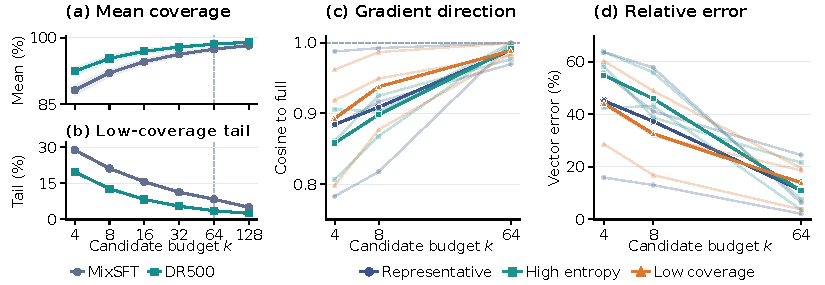
\includegraphics[width=\linewidth]{figures/layout_followup_20260918/smollm_supervision.pdf}
\caption{\textbf{Larger candidate sets improve coverage and gradient approximation in SmolLM.}
(a,b) Mean retained student probability and fraction of inputs below 90\% coverage; bands show response-cluster 95\% intervals. Dashed lines mark top-64.
(c,d) Gradient cosine and relative error against full-vocabulary supervision at the trained student. Groups comprise typical inputs, uncertain next-token predictions, and inputs with lower top-64 coverage; thin lines show batches and bold lines their means. MixSFT/DR500 denote the initialization/trained student. Protocol details appear in Appendix~\ref{app:smollm_diagnostics}.}
\label{fig:smollm_supervision}
\end{figure}

These measurements make coverage and gradient error useful checks for a chosen vocabulary budget. Each model's results apply to its teachers and generated responses; the within-model comparisons hold inputs fixed when varying the objective. Appendix~\ref{app:smollm_capability} adds task-level evaluations of the SmolLM students.
